\section{Calibrated joint tests of generator predictions}
\label{sec:joint5d}

% Campaign: s5p (terminal 2026-10-06).
This section is the complete record of the joint five-dimensional generator
tests, whose design was fixed before any production pseudo-experiment or
observed statistic, with two disclosed data-informed elements
(\S\ref{sec:joint5d-frozen}); the article states
its result and conditions and refers here for the detail. The tests evaluate
simple hypotheses about five predictions. They are not a measured cross
section, add no reportable uncertainty (App.~\ref{app:provenance},
\texttt{joint-5d}), and do not re-qualify the adopted five-axis covariance of
\S\ref{sec:eavailw-adopted}, which they do not use. The frozen contract and
recorded result are in Ref.~\cite{JointTestRecord2026}.

\subsection{Hypotheses, grid and statistics}
\label{sec:joint5d-design}

For each of five predictions $G$ (the MINERvA Tune~v1, GENIE~2.12.10 without
and with MEC, NuWro~21.09 and GiBUU~2019; \S\ref{sec:eavailw-band}), the null
$H_{0}(G)$ is that the true cross section equals $G$ on a fine
five-dimensional grid, with the Tune~v1's shape and $G$'s finite-sample
fluctuations below that grid. This \emph{hybrid null} is the hypothesis the
calibration simulates; for the Tune~v1, the analysis simulation itself, it is
$H_{0}$ exactly. Each prediction is tested in total (rate and shape together)
and in shape alone: \jtNtests{} tests.
% plain-language pass 2 (DECISION-20261018-joseph-plain-language-pass2): pass-1 paper F7, note home first.
% Source: nd-unfolding/s5p_stage1_inspect.py:38-44 (FINE, the edges of sec_method.tex:270-275, beside J_EDGES,
% the coarse test grid below); RC4 fine-to-J map U (109, 65856), 65856 = 14*16*7*7*6,
% docs/publication/audit-20261008/notes/mapping-notes-C.md:25.
The fine grid is the analysis binning of \S\ref{sec:method-binning},
$14\times16\times7\times7\times6$ bins in $(\pT,\pPar,\Eavail,q_{3},W)$; the
test cells below are its integrals.

The tests are evaluated on a coarse $3^{5}$ grid in
$(\pT,\pPar,\Eavail,q_{3},W)$ with edges
$\pT\in[0,0.55,0.85,4.5]\,\si{GeV/c}$, $\pPar\in[1.5,3.5,6,60]\,\si{GeV/c}$,
$\Eavail\in[0,0.4,1.5,100]\,\si{GeV}$, $q_{3}\in[0,1.2,2,100]\,\si{GeV}$ and
$W\in[0,1.4,2.2,100]\,\si{GeV}$, restricted to the \jtNcells{} supported
cells (J); for GiBUU, whose sample lacks high-energy neutrinos, the domain is
the \jtNcellsGiBUU{} cells with $\pPar<\SI{6}{GeV/c}$. The grid specifies a
finite hybrid hypothesis and a reporting statistic; it does not turn
OmniFold's event-level training into binned unfolding.

Two statistics are formed from the unfolded cell values $F$ and the
prediction $\mu_{G}$: a total statistic $T_{\mathrm{tot}}=r^{\top}\Sigma^{-1}r$
with $r=F-\mu_{G}$, and a shape statistic $T_{\mathrm{sh}}$ of the same form
on the normalized cell fractions, with the normalization Jacobian applied to
$\Sigma$ and one cell dropped. The metric
$\Sigma=V+\mathrm{diag}\,\mathrm{Var}(\mu_{G})$ adds the prediction's own
finite-sample variance to $V$, a Ledoit--Wolf-shrunk
covariance~\cite{LedoitWolf:2004} of \jtVn{} pilot pseudo-experiments at the
Tune~v1 null. The metric defines how hypotheses are compared and so affects
power; the null calibration below, not the metric, sets each test's size.

\subsection{Calibration through the full analysis chain}
\label{sec:joint5d-calibration}

The null distribution of each statistic is obtained from pseudo-experiments
that run the full analysis chain at the null truth, using the joint-test
estimator (\S\ref{sec:val-departure}: deterministic LightGBM OmniFold, five
iterations, negative-weight background treatment with a 400-tree, 31-leaf
refinement classifier, chosen before the design was frozen). Each
pseudo-experiment
\begin{itemize}[itemsep=1pt, topsep=2pt]
  \item draws Poisson pseudo-data from one half of the simulation together
        with an independent background source, refits the
        background-refinement classifier, and unfolds with the estimator
        trained on the other half;
  \item draws one of \jtFluxUniverses{} flux universes and every one of the
        \jtModelBands{} interaction-model bands at one of its universes;
  \item draws the weight-based detector bands (MINOS muon-matching efficiency
        and the GEANT4 neutron, pion and proton interaction reweights) and the
        five muon and beam-angle lateral bands through a linear surrogate;
  \item draws a \SI{1.4}{\percent} normalization, the data's rounding noise
        (taken from 20 real-data re-unfolds with rounding-level input changes),
        and the prediction's finite-sample residual.
\end{itemize}
The data are unfolded once, with the full simulation. The Monte Carlo $p$ value
of a test is $(k+1)/(B+1)$, where $k$ of $B$ null pseudo-experiments reach the
observed statistic; it is never zero. The \emph{claim} $p$ value is the largest
over declared variants that move the null by an upper bound on the
simulation-size difference between the pseudo-experiments and the data unfold
(condition~(iv) below) and by $\pm\jtMoneKappa\,\delta_{\mathrm{fine}}$
(condition~(i)). The external nulls are strongly non-central, with
non-centralities $\lambda$ of \jtLambdaMin{}--\jtLambdaMax{} in these units,
because the calibration reproduces the estimator's pull toward its prior
(\S\ref{sec:val-departure}); each observed statistic is compared with that
displaced distribution (Fig.~\ref{fig:joint5d-nulls}).

\subsection{Multiplicity, stopping rule and the frozen design}
\label{sec:joint5d-frozen}

The ten tests are controlled at familywise level $\alpha=\jtAlpha$ by the Holm
procedure~\cite{Holm:1979}: under the testing assumptions, the probability of
falsely rejecting at least one true hypothesis among the ten is at most 5\%. A
determinacy requirement also applies: a step rejects only when the 95\%
Clopper--Pearson interval~\cite{Clopper:1934} of $k/B$ lies entirely below its
Holm threshold. Calibration proceeded in batches of \jtBatch{}
pseudo-experiments per null, to at most \jtBcap{}, under a sequential rule
that stopped a null once both of its decisions were determined.

The hypotheses, statistics, variants, multiplicity rule, stopping rule and
every input were frozen before any production pseudo-experiment or observed
statistic. Two data-informed elements are disclosed. Reviewers of the design
had seen descriptive per-cell residuals before it was frozen, and the job
controller's status outputs exposed observed claim $p$ values during
production. A bounded extension of the production budget was decided while
they were visible, to let the sequential rule reach its frozen stop rather
than a budget stop. No statistic, variant, threshold or stopping rule was
changed, and the Monte Carlo $p$ values remain valid at the number of
pseudo-experiments reached. An independent recomputation of every $p$ value
and decision from the stored products, with separately written code, agrees
with the production evaluation on all \jtRecompRows{} compared rows; it
verifies the calculation, not the adequacy of the calibration.

\subsection{Conditions}
\label{sec:joint5d-conditions}

Each decision holds under six conditions of the declared model, numbered as in
the frozen contract and grouped here by kind.

\paragraph{Numerical convergence.}
(i) Below the fine grid the null truth carries the Tune~v1's shapes, and the
fine-grid convergence check has not shown convergence. In the $L_{2}$ norm of the
per-cell relative changes, the last refinement, from a twofold-merged grid to
the fine grid, is \jtMoneMin--\jtMoneMax{} of the whole change from the coarse
test grid to the fine grid, so in that norm the steps are not shown to shrink
and the residual below the fine grid is unmeasured and potentially material.
The frozen design takes the step in a proxy of the test metric to shrink by
\jtMoneWnormMin--\jtMoneWnormMax{} per halving, a design-review value whose
calculation is not recorded. If it kept shrinking geometrically at that rate,
the residual would be about one to three times the last step,
$\delta_{\mathrm{fine}}$ (the change of the noise-free unfolded result when the
null truth is refined from the twofold-merged grid to the fine grid). This sets
the claim variants at $\pm\jtMoneKappa\,\delta_{\mathrm{fine}}$, the central
extrapolated estimate, and the report-only robustness check at
$\pm\jtMoneKappaRobust\,\delta_{\mathrm{fine}}$. The extrapolation assumes
geometric convergence; the measured $L_{2}$ ratios also allow slower rates and
larger residuals. Measured before any observed statistic, the claim variants
move the external nulls by \jtMoneClaimSdMin--\jtMoneClaimSdMax{} null
standard deviations and the robustness variants by
\jtMoneRobSdMin--\jtMoneRobSdMax{}. For the hybrid null as simulated the
residual plays no role; the variants carry the rejections over to $G$ itself
only if replacing the Tune~v1's shape below the fine grid by $G$'s moves the
noise-free unfolded result by no more than $\pm\jtMoneKappa\,\delta_{\mathrm{fine}}$
along $\delta_{\mathrm{fine}}$. (vi) The predictions' own finite samples enter
the metric as $\mathrm{diag}\,\mathrm{Var}(\mu_{G})$ and the simulated
residuals as a drawn term.

\paragraph{Calibration validity.}
The Monte Carlo $p$ values are exact for the simulated null to the extent that
the pseudo-experiment chain reproduces the analysis applied to the data. Two
known departures are bounded. (iv) The pseudo-experiments unfold with half of
the simulation and the data with all of it; the resulting shift, at most about
0.07 null standard deviations but not always consistent with zero, enters as
the bias-aligned upper-bound variant. The data unfold's rounding-level
nondeterminism, measured over the 20 re-unfolds, leaves every observed $p$ value
unchanged except NuWro's shape test (2/1752 to 3/1752).
% 0.07: the frozen-V prefreeze measurement (max 0.068, GENIE+MEC), which supersedes amendment 7 condition 4's
% reviewer-proxy "~0.05" (docs/publication/audit-20261008/CLAIM-TABLE-20261008.tsv row J12;
% REVIEW-20261007-paper-completion.md E6). This section printed 0.05 until 2026-10-11.

\paragraph{Physical-model adequacy.}
(ii) The detector model is the simulation's, varied only by the drawn detector
bands and the linear surrogate for the lateral bands. The analysis has no band
for the calorimetric recoil-energy response, so completeness of the
hadronic-response model is not established (\S\ref{sec:joint5d-response}).
(iii) The interaction-model prior is the analysis's \jtModelBands-band set,
every band drawn in every pseudo-experiment; negative weights in two of them
(\texttt{LowQ2\_1}, \texttt{HighQ2\_1}) are clipped per universe, at most
0.35\% of a band's shift. (v) GiBUU lacks $E_{\nu}>\SI{20}{GeV}$, and its
out-of-domain truth enters the migrations into its domain; for all
predictions $E_{\nu}>\SI{100}{GeV}$ is absent, which is negligible. The use of
the Tune~v1's shapes below the fine grid in (i) is also a modelling choice of
this kind.

\subsection{Decisions}
\label{sec:joint5d-results}

Table~\ref{tab:joint5d} lists the ten decisions. Every test is rejected at
familywise $\alpha=\jtAlpha$; nine have $k=0$, and NuWro's shape test has
$k=1$. Each rejection also survives the robustness variants at
$\pm\jtMoneKappaRobust\,\delta_{\mathrm{fine}}$, the upper end of the
extrapolation in condition~(i). Figure~\ref{fig:joint5d-nulls} shows each
null's calibrated distribution with the observed statistic: the Tune~v1 null
is centred at small values, whereas the external nulls are displaced far upward
by the estimator's pull toward its prior.

\begin{table}[htbp]
  \centering
  \small
  \begin{tabular}{@{}llrrlll@{}}
    \toprule
    $G$ & test & $B$ & $k$ & claim $p$ & Holm thr. & 95\% CP interval of $k/B$ \\
    \midrule
    NuWro 21.09 & total & 1751 & 0 & 1/1752 & 0.005 & $[0, 0.00210]$ \\
    GENIE~2.12.10 & total & 1366 & 0 & 1/1367 & 0.00556 & $[0, 0.00270]$ \\
    GENIE~2.12.10 & shape & 1366 & 0 & 1/1367 & 0.00625 & $[0, 0.00270]$ \\
    MINERvA Tune~v1 & total & 1365 & 0 & 1/1366 & 0.00714 & $[0, 0.00270]$ \\
    MINERvA Tune~v1 & shape & 1365 & 0 & 1/1366 & 0.00833 & $[0, 0.00270]$ \\
    GiBUU 2019 & total & 1351 & 0 & 1/1352 & 0.01 & $[0, 0.00273]$ \\
    GiBUU 2019 & shape & 1351 & 0 & 1/1352 & 0.0125 & $[0, 0.00273]$ \\
    GENIE~2.12.10 + MEC & total & 1343 & 0 & 1/1344 & 0.0167 & $[0, 0.00274]$ \\
    GENIE~2.12.10 + MEC & shape & 1343 & 0 & 1/1344 & 0.025 & $[0, 0.00274]$ \\
    NuWro 21.09 & shape & 1751 & 1 & 2/1752 & 0.05 & $[0.0000145, 0.00318]$ \\
    \bottomrule
  \end{tabular}
  \caption{Joint five-dimensional generator tests, in Holm order; every test is
  rejected. $B$ is the number of completed calibration pseudo-experiments at
  the frozen stop (1400 submitted per null, NuWro 1800; the rest were lost to
  time limits and recovered report-only, \S\ref{sec:joint5d-lost}), and $k$
  the number at least as extreme as the data; claim $p=(k+1)/(B+1)$ is never
  zero.}
  \label{tab:joint5d}
  % Source: RECORD-20261005-s5p-joint-5d-inference-result.md sec. 2, joint-evaluate.json sha256 b9604502...;
  % robustness: robust-labels.json 206655f9...
\end{table}

\begin{figure}[tbp]
  \centering
  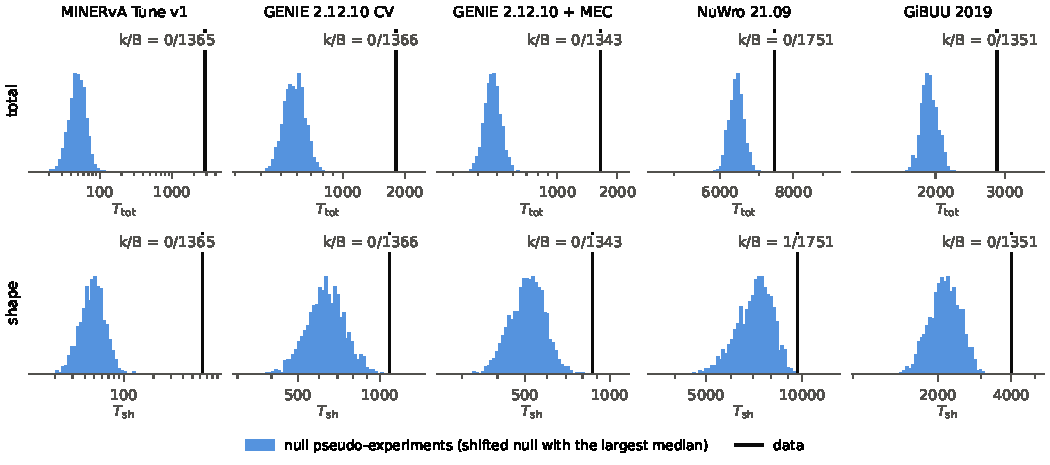
\includegraphics[width=\textwidth]{paper_joint_nulls}
  \caption{Calibrated null distributions of the joint statistics for each
  prediction (columns), total statistic (top) and shape statistic (bottom),
  shown for the declared claim variant whose null distribution has the largest
  median; the vertical line is the observed statistic and $k/B$ is as in
  Table~\ref{tab:joint5d}. The horizontal axis is logarithmic. Plotted from
  the released sufficient inputs (App.~\ref{app:release}), which reproduce
  every recorded $p$ value and decision.}
  \label{fig:joint5d-nulls}
\end{figure}

\paragraph{Sensitivity to the sub-fine-grid residual.}
\label{sec:joint5d-kappa}

The multiplier $\kappa$ scales the last measured refinement change
$\delta_{\mathrm{fine}}$: $\kappa=1$ means one such change, not one standard
deviation or a confidence level. A report-only scan along the frozen direction
$\delta_{\mathrm{fine}}$~\cite{JointTestKappa2026} found all ten decisions to
remain determinate rejections at every sampled multiplier up to 5.25 in the
frozen ensembles. Determinate rejection is first lost between the sampled
multipliers 5.2547 and 5.2563 (between 5.1688 and 5.1703 with the recovered
draws included), by the GENIE~2.12.10 + MEC shape test, whose interval then
contains its Holm threshold, and, through the Holm step-down, by the
GENIE~2.12.10 shape test; neither is then a determinate failure to reject. The
scan probes one prescribed direction; it establishes neither convergence nor a
bound on the actual below-grid residual, which remains unmeasured and
potentially material.

\paragraph{Power.}
\label{sec:joint5d-power}

Every test rejects, so power is context only (the contract attaches power to
non-rejections). At the Tune~v1 null, two of the three declared alternatives
are detected in shape with power 1.0 at the 0.005 level, and the third, a
MEC-like $(\Eavail,W)$ shape, with \jtPowPthree. At the GENIE~2.12.10 null the
shape powers at 0.005 are \jtPowPonegShape, 0.02 and 0.00. These come from the
frozen sets, each of which lost some of its 200 alternatives to time limits
(172--199 retained). Against the frozen null ensembles, the complete power sets
recovered as in \S\ref{sec:joint5d-lost} agree within 0.01; with the null recomputed on all draws, the first
GENIE~2.12.10 set moves to 0.72.

\subsection{Lost pseudo-experiments and their recovery}
\label{sec:joint5d-lost}

Scheduler time limits interrupted or prevented \jtLostCal{} of the submitted
calibration pseudo-experiments (\jtLostInterrupted{} interrupted,
\jtLostNever{} never started) and \jtLostPow{} power pseudo-experiments, so the
decisions in Table~\ref{tab:joint5d} were evaluated on the completed draws. A
sensitivity computed before the lost outcomes were known showed that every
decision could change under a realizable assignment of them: had every
interrupted draw exceeded the observed statistic, no test would have been
rejected ($p$ \jtWorstIntLo--\jtWorstIntHi). Among completed draws, runtime is
not associated with the statistic ($|\rho|\le\jtRuntimeRho$), which supports
but does not certify the decisions.

The lost seeds were therefore rerun, report-only, under a procedure fixed and
independently reviewed beforehand~\cite{JointTestRecovery2026}. A determinism
check fixed in advance (16 of 16 completed seeds rerun bitwise identically)
shows that each recovered draw is the lost draw, so every submitted draw has
now been observed. No recovered draw reaches the observed statistic in any
test, claim variant or robustness variant, so no assignment of the lost draws
changes any decision. The closest margin is 4.6 units of $T$ below the observed
value of 868.6 (GENIE~2.12.10 + MEC shape, $\pm\jtMoneKappaRobust\,\delta_{\mathrm{fine}}$
variant); the next is 49.8 (GENIE~2.12.10 shape, same variant). With complete
batches the frozen rule would have stopped the Tune~v1, GENIE~2.12.10,
GENIE~2.12.10 + MEC and GiBUU nulls one batch earlier ($B=1200$), with the same
decisions.

The scope of the recovery's checks is narrower than that of the main
recomputation:
\begin{itemize}[itemsep=1pt, topsep=2pt]
  \item its independent cross-check (856 of 856 quantities) covers only the
        reading with the frozen variant shifts;
  \item the reading with the recovered draws added to the calibration (the
        shift recomputed on all draws) was reproduced only by a standalone
        replay of the same code, a consistency check rather than an
        independent recomputation;
  \item the earlier-stop decisions rest on the campaign's self-validated
        re-application of the sequential rule.
\end{itemize}
The recovery is report-only: the primary decisions are those of the frozen
evaluation, at the frozen $B$, and the recorded disposition of the recovery
is ``certified, margin disclosed''.
% Source: RECORD-20261006-s5p-lost-seed-recovery-resolution.md (recovery, margins 4.6/49.8 T units, earlier
% stops, power over the complete sets); RECORD-20261005 sec. 5 (pre-recovery sensitivity, |rho| <= 0.06);
% DECISION-20261005-s5p-recompute-extension-and-lost-seed-recovery.md sec. 5 (Joseph's disposition).

\subsection{Matched coarse projections}
\label{sec:joint5d-projections}

Restricting the same calibrated tests to matched $3\times3$ coarse projections
of the same cells, onto $(\pT,\pPar)$ and onto $(\Eavail,W)$, gives $p<0.05$
for every test in at least one of the two projections, so this study provides
no evidence of additional discrimination from the joint five-observable
information. The comparison was specified before it was run but after the
five-dimensional outcomes were known; it uses the same calibration ensembles,
with the recovered draws included, and the same variants and claim rule, and
its $p$ values were reproduced independently~\cite{JointTestProjections2026}.
In the muon-only $(\pT,\pPar)$ projection, GENIE~2.12.10 is not rejected
($p=\woneGcvPtTot$ in total, $\woneGcvPtShape$ in shape; a post hoc
observation), whereas its $(\Eavail,W)$ projection is. Hadronic information
therefore participates in that rejection; this does not establish added power
of the joint test over all matched projections, or accept GENIE as true.

\subsection{Hadronic-response condition and recoil-energy sensitivity}
\label{sec:joint5d-response}

MINERvA's recoil-energy analyses assign a hadronic-energy response uncertainty
derived from test-beam calorimetry~\cite{MINERvA:2015testbeam}, separate from
the GEANT hadron-interaction reweights~\cite{MINERvA:2021owq,MINERvA:2022incl};
in the low-recoil measurement the resulting hadronic-energy uncertainty rises
to \SI{10}{\percent} at its highest three-momentum transfers,
$0.9<q_{3}<\SI{1.2}{GeV}$~\cite{MINERvA:2022incl}. The declared nuisance model
here includes the reweights but no calorimetric response band. Such a band
would act on all five nulls together, through the shared detector simulation
and unfolding: a response mismodelling could move each observed statistic in
either direction, and a band drawn in the calibration would also broaden and
could shift each null distribution; the net effect on each $p$ value is
unmeasured. The published comparison in muon kinematics alone, whose
observables do not use the reconstructed recoil energy, also disfavours the
same generator families~\cite{MINERvA:2021owq}; it provides context for a
disagreement involving muon observables, but the hypotheses tested here use a
different estimator and calibration. The GENIE~2.12.10 projection result of
\S\ref{sec:joint5d-projections} shows that the information rejecting that
prediction involves the hadronic axes, on which a response band would act.

For an exploratory response sensitivity study~\cite{JointTestRecoil2026}, the
data are re-unfolded with the simulation's reconstructed recoil energy scaled
by $\pm\SI{4}{\percent}$, and the frozen tests are re-evaluated against the
frozen null distributions. The size is the level of data--simulation agreement
reported for test-beam protons, pions and electrons of
0.35--\SI{2.0}{GeV/c}~\cite{MINERvA:2015testbeam}; neutrons and
higher-momentum hadrons, which matter at high $W$, lie outside that sample.
The $\pm4\%$ size is a labelled exploratory sensitivity, not a validated
uncertainty prescription. A re-unfold with unscaled recoil reproduces
the frozen decisions, with every claim $p$ value inside the range spanned by
the data's rounding variations. At both $-4\%$ and $+4\%$ every one of the ten
rejections holds. The observed statistics move by up to about \SI{11}{\percent}
from their frozen values, nine tests keep $k=0$, and NuWro's shape test, the
closest to its null, changes from $k=1$ to $k=3$ of 1751 at $+4\%$
($p=0.0023$, against a Holm threshold of 0.05). The evaluation was reproduced
independently.

The calibration distributions stay fixed in this study, which measures the
sensitivity of the observed statistics and decisions to one coherent scale of
reconstructed available energy and recoil energy, applied after the energy
calibration at a single magnitude. A response-uncertainty construction would
also need to vary the null distributions. The study leaves untested (a) the
response of the null distributions, which were not regenerated with the
variation although they are simulated through the same detector model, so the
size of this omission is unmeasured for these strongly non-central nulls;
(b) particle-species, energy-dependent or resolution effects, and a response
difference applied before calibration; and (c) larger variations. The
rejections are therefore conditional on the simulation's hadronic response,
and the response model is not shown to be complete.

\subsection{What the tests establish}
\label{sec:joint5d-reading}

The comparisons recover the generator disagreements already established by
the published two-dimensional measurement on the same
data~\cite{MINERvA:2021owq}. Their methodological contribution is calibration
through the full analysis chain, which puts the estimator's bias toward its
prior and the declared nuisances into each null distribution. The rejections
are global assessments of the five specified predictions under the declared
model; assigning a discrepancy to a kinematic region or nuclear mechanism
would require separate tests. They apply to the generator versions listed in
\S\ref{sec:eavailw-band} and retain all six conditions of
\S\ref{sec:joint5d-conditions}; in particular, the hadronic response and the
sub-fine-grid residual remain outside any validated uncertainty bound.
Extending the inference would require a response band drawn through the
calibration and a demonstrated bound on the residual below the fine grid.
% Source: docs/orchestration/RECORD-20261005-s5p-joint-5d-inference-result.md (decisions, B, k, p, the six
% conditions); DELIVERY-20261006-s5p-campaign-terminal.md; W1 (docs/publication/w1/W1-RECORD-20261006.md);
% W2 (publication/w2/W2B-REPORT-20261006.md); kappa (publication/kappa/RECORD-20261008-kappa-breakdown.md).
% Section assembled 2026-10-11 from the article's former Sec. VI and the note's former sec_eavailw subsection,
% when the article's joint-test section was shortened.
